\documentclass[12pt,a4paper]{article}
\usepackage[utf8]{inputenc}
\usepackage{graphicx}  
\usepackage{amsmath}
\usepackage{amsfonts}
\usepackage{amssymb}
\usepackage{gensymb}  % degree symbols
\author{Richard Decal}
\title{%
  Solving Cartpole Using Reinforcement Learning and Policy Gradients \\
  \large Machine Learning Engineer Nanodegree\\
  Capstone Project}
\usepackage[style=numeric,sorting=none]{biblatex}
\addbibresource{references.bib}
%\bibliographystyle{unsrt}

\begin{document}

\maketitle


\section{Definition}
%_(approx. 1-2 pages)_

\subsection*{Project Overview}
%In this section, look to provide a high-level overview of the project in layman’s terms. Questions to ask yourself when writing this section:
%- _Has an overview of the project been provided, such as the problem domain, project origin, and related datasets or input data?_
%- _Has enough background information been given so that an uninformed reader would understand the problem domain and following problem statement?_

Reinforcement learners are a class of algorithms which learn to perform a task by taking actions and recieving feedback from its environment. The algorithm uses the feedback to optimize its behavior to maximize future rewards. These algorithms can amazingly become proficient at a given task-- outperforming humans in some domains-- without ever being given explicit directions, rules, explanations, or any domain knowledge whatsoever. Given enough time to test various strategies, a good reinforcement learning algorithm will converge to the optimal decision policy.

In this work, I will use reinforcement learning to solve ``CartPole", a classic control problem with a binary choice at each timestep. This problem was first solved using neural network-like algorithms in 1983.\cite{og_cartpole} Reinforcement learning is capable of learning this task due to its relatively small state and output spaces.\cite{deep_pg}\cite{ddpg_blog}

\subsection*{Problem Statement}
%In this section, you will want to clearly define the problem that you are trying to solve, including the strategy (outline of tasks) you will use to achieve the desired solution. You should also thoroughly discuss what the intended solution will be for this problem. Questions to ask yourself when writing this section:
%- _Is the problem statement clearly defined? Will the reader understand what you are expecting to solve?_
%- _Have you thoroughly discussed how you will attempt to solve the problem?_
%- _Is an anticipated solution clearly defined? Will the reader understand what results you are looking for?_

``CartPole" is a simple 2D game which simulates an upright pole connected by a hinge to a cart.\cite{cartpole} The cart moves freely on a frictionless surface. Each trial is initiated with the cart at the center of the environment and the pole upright. At each timestep, the agent has to choose between pushing the cart to left or to the right. The trial ends if the pole tilts 15$\degree$ away from vertical, if the cart has translated to the edge of the screen, or if the trial reaches its time limit. For each timestep in a trial, the game rewards the player +1 point.

The goal is to train an algorithm which can maintain the pole upright and within bounds for all 200 timesteps.

\subsection*{Metrics}
%In this section, you will need to clearly define the metrics or calculations you will use to measure performance of a model or result in your project. These calculations and metrics should be justified based on the characteristics of the problem and problem domain. Questions to ask yourself when writing this section:
%- _Are the metrics you’ve chosen to measure the performance of your models clearly discussed and defined?_
%- _Have you provided reasonable justification for the metrics chosen based on the problem and solution?_

The most salient metric is episode length, as the game is defined as solved when the algorithm can stay ``alive" until the time limit.

The second metric will be histograms of the pole's angle $\theta$. We expect these to collapse to a single peak near zero (corresponding to an upright pole) for an optimal policy.

Initially, I created a bonus system to reward states with the pole upright and the cart close to the center of the track, with the rational that these are states which are least likely to lead to failure. However, I disabled those because they amounted to injecting my domain knowledge into the reward system, and I thought it would be more interesting to create an algorithm which learned good states from a completely naive starting point. In addition, some trajectories full of bad decisions, which lasted a very short time, might get a relatively high score because the game ended quickly and the average $x$ and $\theta$ were relatively low, wheras a 

Finally, one might expect to examine the discounted rewards which the agent actually uses to judge its own performance of a trial. However, as we will see later, these have been mean subtracted and scaled down to unit variance. The effect is that all early timesteps are always punished, and all timesteps near the absorbing state are punished all the time. This turns out to be sufficient for converging, but cannot be used as a metric for comparison in a meaninful way.
%
However, if all actions are equally labeled as being worth +1 rewards, the algorithm has no way of descriminating between good actions and bad actions. Internally, this was achieved by using Bellman's eqations, which compounds rewards
%
%In order to do that, we have to assign credit to actions that lead to good outcomes in the future. To do this, we give the algorithm discounted rewards instead of simply rewards. Discounted rewards are computed using Bellman's Equation:
%
%Discounted rewards are a way of projecting consequences of future states to actions taken in the past. This is done by discounting the future
%
%I will use total discounted rewards as well as average discounted reward per timestep as metrics. While these are not in themselves are true objective, they are the external signals that the algorithm actually uses to formulate the gradients used to optimize its decision policy. 

\section{Analysis}
%_(approx. 2-4 pages)_
%
\subsection*{Data Exploration}
%In this section, you will be expected to analyze the data you are using for the problem. This data can either be in the form of a dataset (or datasets), input data (or input files), or even an environment. The type of data should be thoroughly described and, if possible, have basic statistics and information presented (such as discussion of input features or defining characteristics about the input or environment). Any abnormalities or interesting qualities about the data that may need to be addressed have been identified (such as features that need to be transformed or the possibility of outliers). Questions to ask yourself when writing this section:
%- _If a dataset is present for this problem, have you thoroughly discussed certain features about the dataset? Has a data sample been provided to the reader?_
%- _If a dataset is present for this problem, are statistics about the dataset calculated and reported? Have any relevant results from this calculation been discussed?_
%- _If a dataset is **not** present for this problem, has discussion been made about the input space or input data for your problem?_
%- _Are there any abnormalities or characteristics about the input space or dataset that need to be addressed? (categorical variables, missing values, outliers, etc.)_

For this task, my learner will be totally naive and will have no previous data to inform the policy. The game environment has a convenient open-source wrapper provided by OpenAI which allows us to step through trials.\cite{cartpole} At each timestep, the game provides the agent the current environment state as well as the reward for the action taken at the previous timestep.  The sensory input is the cart's position $x$, the cart's velocity $\dot x$, the pole's angle $\theta$ (measured in radians), and its rate of change $\dot\theta$.\cite{state_def} 

Given the state and the chosen action, the agent is given immediate feedback from the game in the form of a reward. These (state, action, reward) pairs are crucial for the reinforcement algorithm to improve its policy from its experiences (discussed in the project design section).

I initially thought of reducing the state space to simply the $x$ position and $\theta$. However, the problem with that is the agent has no way of knowing from a single frame whether the speed at which the pole and cart are moving. If the system is rapidly moving in one direction, it is important for the agent to oppose that movement to cancel it out, or otherwise the episode will end. For instance, if at a given state the pole is slightly tilted, the 2-state agent would naively think it should push it towards the vertical. However, if the pole is already rapidly swinging towards the vertical, accelerating it even more would make in impossible to then stop it from swinging too far the other way. The correct action would have been to anticipate this and oppose to pole. Since the integral of force is mometum, these kinematic values are effectively a kind of memory for the agent. 



%\subsection*{Exploratory Visualization}
%In this section, you will need to provide some form of visualization that summarizes or extracts a relevant characteristic or feature about the data. The visualization should adequately support the data being used. Discuss why this visualization was chosen and how it is relevant. Questions to ask yourself when writing this section:
%- _Have you visualized a relevant characteristic or feature about the dataset or input data?_
%- _Is the visualization thoroughly analyzed and discussed?_
%- _If a plot is provided, are the axes, title, and datum clearly defined?_
%
\subsection*{Algorithms and Techniques}
%In this section, you will need to discuss the algorithms and techniques you intend to use for solving the problem. You should justify the use of each one based on the characteristics of the problem and the problem domain. Questions to ask yourself when writing this section:
%- _Are the algorithms you will use, including any default variables/parameters in the project clearly defined?_
%- _Are the techniques to be used thoroughly discussed and justified?_
%- _Is it made clear how the input data or datasets will be handled by the algorithms and techniques chosen?_

I tried various reinforcement algorithms in the course of the project. Initially, I attempted to use an actor critic network. The name refers to the two neural networks which comprise the algorithm: a critic network and an actor network. The critic takes a series of (state, action) pairs and outputs a reward vector, wheras the actor takes states as an input and computes the probability it should take different actions. The actor's optimizer tries to maximze the rewards it will recieve from the critic. 

I also tried a policy gradient algorithm without a critic network. In place of the critic network, I passed the environemental rewards through Bellman's Equation to get discounted rewards (discussion in the ``implementation" section). These discounted rewards were then used to calculate the loss for each particular action, and an Adam optimizer was used to minimze the loss.

The actor-only algorithm is much simpler due to the fact that it is comprised of only one neural network instead of two. The actor network takes states and outputs action probabilities. The network is comprised of one or more fully connected layers, which are then passed through a sigmoid activation function.

Specifics about implementation of these algorithms are discussed in ``Implementation" section.


\subsection*{Benchmark}
%In this section, you will need to provide a clearly defined benchmark result or threshold for comparing across performances obtained by your solution. The reasoning behind the benchmark (in the case where it is not an established result) should be discussed. Questions to ask yourself when writing this section:
%- _Has some result or value been provided that acts as a benchmark for measuring performance?_
%- _Is it clear how this result or value was obtained (whether by data or by hypothesis)?_
To establish a baseline, I created two simple models to compare my policy gradient algorithm. The first is a random actor, which takes a random action at each timestep. The second is a ``contrarian'' actor. The contrarian actor simply looks at which direction the pole is tilting, and always pushes the pole towards the upright position.

\section{Methodology}
%_(approx. 3-5 pages)_
%
%\subsection*{Data Preprocessing}
%In this section, all of your preprocessing steps will need to be clearly documented, if any were necessary. From the previous section, any of the abnormalities or characteristics that you identified about the dataset will be addressed and corrected here. Questions to ask yourself when writing this section:
%- _If the algorithms chosen require preprocessing steps like feature selection or feature transformations, have they been properly documented?_
%- _Based on the **Data Exploration** section, if there were abnormalities or characteristics that needed to be addressed, have they been properly corrected?_
%- _If no preprocessing is needed, has it been made clear why?_


\subsection*{Implementation}
%In this section, the process for which metrics, algorithms, and techniques that you implemented for the given data will need to be clearly documented. It should be abundantly clear how the implementation was carried out, and discussion should be made regarding any complications that occurred during this process. Questions to ask yourself when writing this section:
%- _Is it made clear how the algorithms and techniques were implemented with the given datasets or input data?_
%- _Were there any complications with the original metrics or techniques that required changing prior to acquiring a solution?_
%- _Was there any part of the coding process (e.g., writing complicated functions) that should be documented?_

I began trying to solve CartPole using an actor-critic model. However, after a few days of work I could not make any progress getting it to learn, no matter which parameters and architectures I tried. In order to make headway on my project, I switched to policy gradients without a critic network, which has less than half the number of parameters and complexity.

Once I switched to the policy gradient algorithm, I tested it with various architectures and hyperparameters. I tested up to four fully conencted layers. I tried between 10 and 200 neurons per layer. I added a dropout layer before the final fully connected layer. I tried various activation functions, tanh, sigmoid, and softmax. A graph of our model is shown on Figure \label{actor_net}. I had also tried using dropout layers and different numbers of hidden layers, but this worked best. Bias.  


Instead of having a neural network representing the reward function, it takes rewards directly from the environment instead, passed through Bellman's Equation (Equation \ref{bellman}).

\begin{equation}\label{bellman}
D(a_i) = R(a_i) + \gamma \sum_{n=i+1}^{\infty}{R(a_n)} 
\end{equation}

The discounted rewards were further processed by subtracting the mean and dividing by the standard deviation. Subtracting the mean promotes actions with higher-than-expected rewards, and penalizes ones that give lower-than-expected rewards. Dividing by the standard deviation made training more stable, since the rewards had much lower variance.

This works fairly well, but the training is very volatile because the discount reward always rewards early actions and penalizes late actions, regardless of which actions were actually chosen. The idea is that, if a trajectory lasts a long time, the early actions will have accumulated quite a large discounted reward. To further reduce variance, I tried two different batching techniques. One is to save all the (state,action,reward) pairs into a replay buffer, and after a certain amount of trials solve the discounted reward across all the different trajectories in the mini batch. The advantage of this is that when we subtract the mean and standard deviation it will be of our entire batch. Thus, each indiviual action are scored against a larger pool of actions and the model can better discriminate between good and bad actions.

Similarly, I tried using batched gradients. During each episode in the batch, we compute the gradient of the loss with respect to our parameters and add it to the running gradient sum vector. We continue to add each computed gradient into the batch gradient. The idea is that, since the rewards are very volatile, any given gradient for any particular parameter might sometimes be positive or negative, but that variance is smoothed out over multiple trials.

Initially, I created a bonus system to reward states with the pole upright and the cart close to the center of the track, with the rational that these are states which are least likely to lead to failure. However, I disabled those because they amounted to injecting my domain knowledge into the reward system, and I thought it would be more interesting to create an algorithm which learned good states from a completely naive starting point.


\begin{figure}[htbp]
\begin{center}
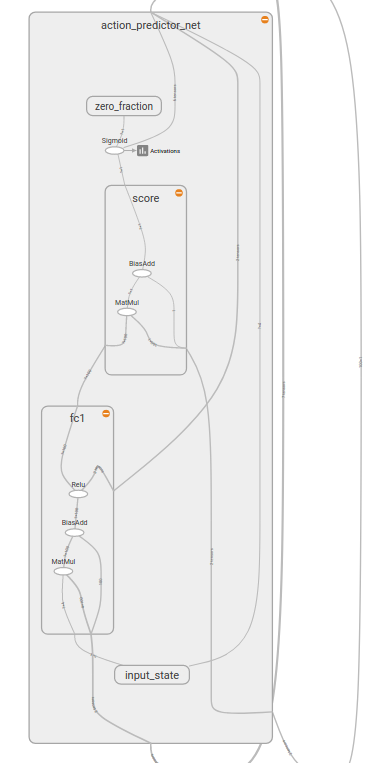
\includegraphics[scale=0.6]{actor_net.png}
\caption{Graph of my finalized actor network architecture. Input state is our observed state for that timestep. fc1 is a fully-connected layer with a ReLu activation. Score is a second fully connected layer. Finally, the scores are given to a sigmoid activation layer which outputs a single value between 0 and 1. This is the probability of choosing ``push right" action at that timestep.}
\label{actor_net}
\end{center}
\end{figure}





more complicated

less complicated. 


everything that used dropout crashed to 10 ts, so I removed that as a param.

new loss function

cross ent

new rewards

experience replay

gradient buffers

softmax of two probabilties --> one probability 


overnight run with actor critic


\subsection*{Refinement}
%In this section, you will need to discuss the process of improvement you made upon the algorithms and techniques you used in your implementation. For example, adjusting parameters for certain models to acquire improved solutions would fall under the refinement category. Your initial and final solutions should be reported, as well as any significant intermediate results as necessary. Questions to ask yourself when writing this section:
%- _Has an initial solution been found and clearly reported?_
%- _Is the process of improvement clearly documented, such as what techniques were used?_
%- _Are intermediate and final solutions clearly reported as the process is improved?_
I finally got a model which trained, but it took 2000 iterations to solve the game.


Tensorboard was invaluable. It allowed easy comparison across multiple models. By the end, I compared dozens of models before selecting the best one. 

I wanted to see how fast my model could converge to a perfect policy.

However, while these find the game quickly, the combination of a high learning rate and a noisy reward signal results in inconsitent results. Sometimes we get a perfect score in as little as 13 trials, but sometimes it takes over 100 episodes to do so using the same exact model parameters. 

parameter sweep

adding layers

as models got better, reduced number of episodes


\section{Results}
%_(approx. 2-3 pages)_
%
\subsection*{Model Evaluation and Validation}
%In this section, the final model and any supporting qualities should be evaluated in detail. It should be clear how the final model was derived and why this model was chosen. In addition, some type of analysis should be used to validate the robustness of this model and its solution, such as manipulating the input data or environment to see how the model’s solution is affected (this is called sensitivity analysis). Questions to ask yourself when writing this section:
%- _Is the final model reasonable and aligning with solution expectations? Are the final parameters of the model appropriate?_
%- _Has the final model been tested with various inputs to evaluate whether the model generalizes well to unseen data?_
%- _Is the model robust enough for the problem? Do small perturbations (changes) in training data or the input space greatly affect the results?_
%- _Can results found from the model be trusted?_

\subsubsection*{Random Policy}
Each episode lasted on average about 
\begin{figure}[htbp]
\begin{center}
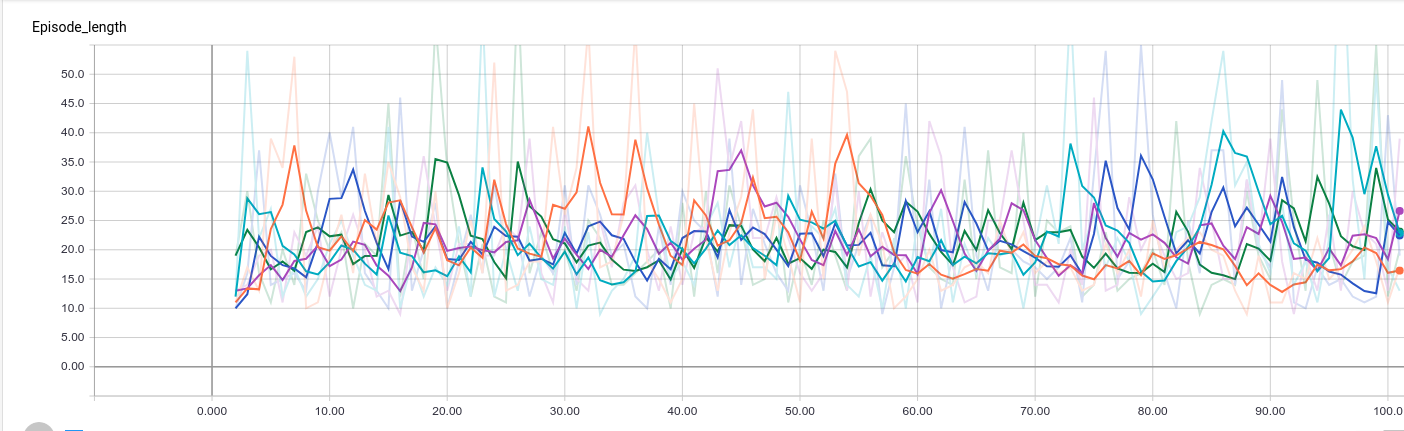
\includegraphics[width=\linewidth]{rand_ep_length.png}
\caption[]{}
\label{rand_ep_length}
\end{center}
\end{figure}
 The distribution of thetas 

\begin{figure}[htbp]
\begin{center}
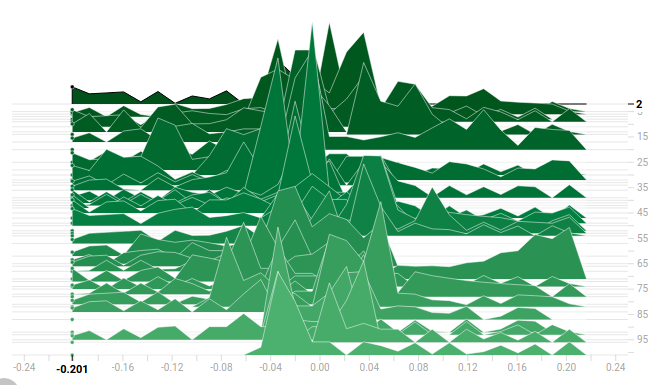
\includegraphics[width=\linewidth]{rand_thetas.png}
\caption{Distribution of thetas for random policy}
\label{rand_ep_length}
\end{center}
\end{figure}

\subsubsection*{Contrarian Policy}

Each episode lasted on average about 
\begin{figure}[htbp]
\begin{center}
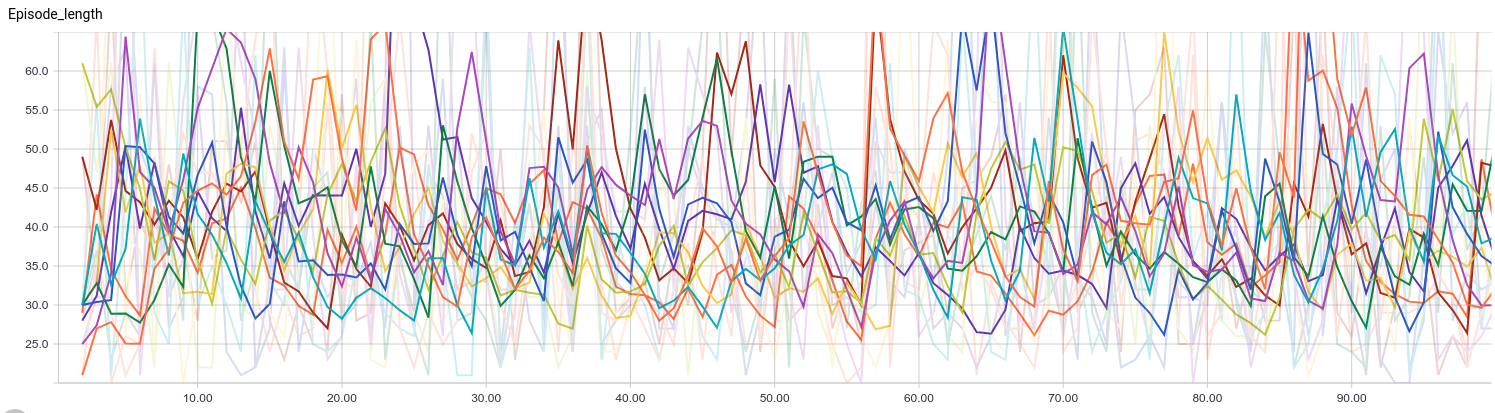
\includegraphics[width=\linewidth]{contrarian_lengths.png}
\caption{}
\label{contrarian_lengths}
\end{center}
\end{figure}

The distribution of thetas 

\begin{figure}[htbp]
\begin{center}
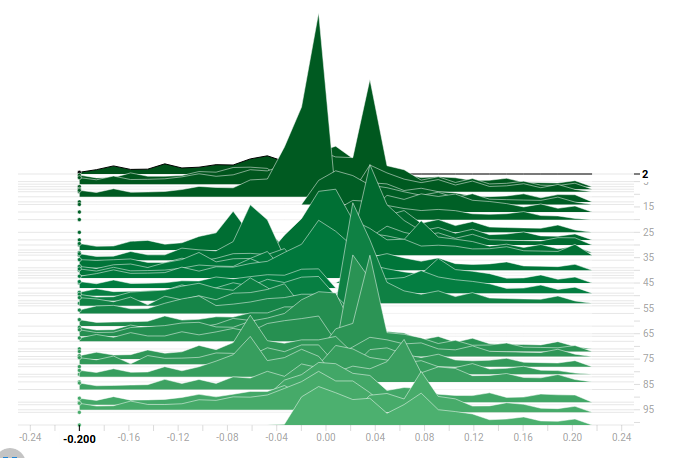
\includegraphics[width=\linewidth]{contrarian_thetas.png}
\caption{Distribution of thetas for contrarian policy}
\label{contrarian_thetas}
\end{center}
\end{figure}

\subsubsection*{Policy Gradient}

\subsection*{Justification}
%In this section, your model’s final solution and its results should be compared to the benchmark you established earlier in the project using some type of statistical analysis. You should also justify whether these results and the solution are significant enough to have solved the problem posed in the project. Questions to ask yourself when writing this section:
%- _Are the final results found stronger than the benchmark result reported earlier?_
%- _Have you thoroughly analyzed and discussed the final solution?_
%- _Is the final solution significant enough to have solved the problem?_


\section{Conclusion}
%_(approx. 1-2 pages)_
%
\subsection*{Free-Form Visualization}
%In this section, you will need to provide some form of visualization that emphasizes an important quality about the project. It is much more free-form, but should reasonably support a significant result or characteristic about the problem that you want to discuss. Questions to ask yourself when writing this section:
%- _Have you visualized a relevant or important quality about the problem, dataset, input data, or results?_
%- _Is the visualization thoroughly analyzed and discussed?_
%- _If a plot is provided, are the axes, title, and datum clearly defined?_
%
If I let it run long enough, it lowers in score. That's because the reward function penalizes things near the end, even if doing well. This is good for fast training, but bad once we have converged.

Prone to catastrophic colapse.
\subsection*{Reflection}
%In this section, you will summarize the entire end-to-end problem solution and discuss one or two particular aspects of the project you found interesting or difficult. You are expected to reflect on the project as a whole to show that you have a firm understanding of the entire process employed in your work. Questions to ask yourself when writing this section:
%- _Have you thoroughly summarized the entire process you used for this project?_
%- _Were there any interesting aspects of the project?_
%- _Were there any difficult aspects of the project?_
%- _Does the final model and solution fit your expectations for the problem, and should it be used in a general setting to solve these types of problems?_
start simple

tensorboard is great

save snapshot after perfect performance




\subsection*{Improvement}
%In this section, you will need to provide discussion as to how one aspect of the implementation you designed could be improved. As an example, consider ways your implementation can be made more general, and what would need to be modified. You do not need to make this improvement, but the potential solutions resulting from these changes are considered and compared/contrasted to your current solution. Questions to ask yourself when writing this section:
%- _Are there further improvements that could be made on the algorithms or techniques you used in this project?_
%- _Were there algorithms or techniques you researched that you did not know how to implement, but would consider using if you knew how?_
%- _If you used your final solution as the new benchmark, do you think an even better solution exists?_
%
%-----------
%
%**Before submitting, ask yourself. . .**
%
%- Does the project report you’ve written follow a well-organized structure similar to that of the project template?
%- Is each section (particularly **Analysis** and **Methodology**) written in a clear, concise and specific fashion? Are there any ambiguous terms or phrases that need clarification?
%- Would the intended audience of your project be able to understand your analysis, methods, and results?
%- Have you properly proof-read your project report to assure there are minimal grammatical and spelling mistakes?
%- Are all the resources used for this project correctly cited and referenced?
%- Is the code that implements your solution easily readable and properly commented?
%- Does the code execute without error and produce results similar to those reported?

\end{document}